\chapter{Runtime Verification with the \RH\ Algorithm}
\label{chap:Runtime Verification with the Rosu-Havelund Algorithm}

We now investigate the suitability of the \RH\ algorithm to runtime verification using realtime monitors.  We start by performing a complexity analysis in section \ref{sec:ComplexityAnalysis} that indicates the algorithm appears to be too time-consuming for real-world use when applied.  Then, we confirm those suspicions by performing a practical performance analysis on an implementation of the algorithm.  The implementation is described in section \ref{sec:RosuHavelundImplementation}, followed by some tests in section \ref{sec:FunctionalTestingRosuHavelund} to ensure the correct functioning of the implementation.  In section \ref{sec:PracticalPerformanceAnalysisOfRosuHavelund} a practical analysis is conducted to ascertain the performance over increasing workload.  We finish by explaining the weakness in the algorithm in section \ref{sec:ScalabilityOfRosuHavelund}.

\section{Complexity Analysis}
\label{sec:ComplexityAnalysis}

The computational cost of the \RH\ algorithm is composed of memory cost and execution cost for the initialisation and evaluation phases of the algorithm.  It depends upon the size of the formula being evaluated and the length of the trace evaluated over.  The size of the formula is the number of subformulae $ | \varphi | $ and the trace length is the number of trace events $ | t | $.

The memory and execution cost of the initialisation phase is simply the cost of constructing the \textit{now} and \textit{next} registers. The memory required for each register is equal to the size of $ \varphi $, and the execution cost increases linearly with the size of $ \varphi $.  Both memory and execution costs of the initialisation phase are O($ | \varphi | $).

Evaluation of the formula over a trace takes place in a loop where each iteration evaluates the formula over a different trace entry until the evaluation has covered all entries.  Each of the individual trace entries gets evaluated against every subformula in the \textit{now} register.  Thus the execution cost rises linearly with the size of the formula multiplied by the length of the trace. It is O($ | t | * | \varphi | $).

The memory cost of the evaluation phase is simply the cost of storing the trace.  Therefore it rises linearly with the length of the trace, i.e.,\ the complexity is O($ | t | $).

However, this describes only the static cost of the evaluation phase; the cost of evaluating the formula once over a trace of finite length.  But when the algorithm gets applied in real-world situations, the system being monitored can run for an indefinite period.  Thus any number of events can occur during the execution life of the algorithm.  When new events occur, they get added to the trace, and the formula must be re-evaluated over the new trace.  The reader should draw their attention now to a significant detail regarding the algorithm.  The loop that iterates through the trace does so in reverse order.  It evaluates the formula over the latest trace entry first and continues until the earliest entry.  Meaning, to correctly evaluate an LTL formula, entries can never be removed from the trace.  This poses two fatal problems:  Firstly, the dynamic memory requirements increase indefinitely because the trace grows, albeit linearly, in length and entries can never be removed.  Secondly, the dynamic execution cost increases indefinitely as the trace grows.  But unlike the memory requirement, the dynamic execution cost grows at a far greater rate.  For example, after a single event has occurred, the formula is evaluated over a trace of length 1.  When a second event occurs the formula is re-evaluated over a trace of length 2.  After the next event, the evaluation is over a trace of length 3, and so on.  To illustrate the point, when ten events occur in succession the formula gets evaluated 1+2+3+4 ... 10, a total of 55 times.

The general formula describing the number of evaluations is $ n(n+1)/2 $ where $ n = | t |$, the length of the trace.  In application, the dynamic execution cost of the algorithm is $$O((n(n+1)/2 * |\varphi |) = O((n^2+n)/2 * | \varphi |) = O(n^2 * |\varphi |) = O(| t |^2 * |\varphi |)$$

Therefore when events occur in succession, it requires $ | t |^2 * | \varphi | $ iterations of the evaluation phase to evaluate the formula over the trace.  Such an algorithm has quadratic complexity and will quickly become too time-consuming to be useful.

\section{Implementation}
\label{sec:RosuHavelundImplementation}

Before implementing the algorithm, we were conscious that further investigation into performance improvements were necessary.  With this in mind, the implementation follows an ad-hoc structure where the intention is simply to have a functioning implementation that is true to the design of the algorithm.  Given that further development was likely, this gave us the opportunity to become familiar with the general implementation challenges presented during the standard implementation.  We intended to leave more elegant solutions to a second development cycle where the algorithm would be improved.  In our experience, a two-cycle development approach is welcome when developing anything new because the challenges are understood better after the first cycle.\\

\noindent The algorithm was developed in Java using the Eclipse IDE.  Download it from here:\\
\indent \url{https://www.eclipse.org/downloads/}\\
\\
Appendix \ref{app:RHCode} provides links to the implementation code. 

\subsection{Syntax of Implemented LTL}

For convenience, our implementation of \RH\ allows LTL formulae to be written as free-text strings and parsed during the initialisation phase of the algorithm.  The description of LTL in chapter \ref{chap:Linear Temporal Logic} uses characters that are not available on a typical computer keyboard.  For this reason, we chose alternative characters to represent the LTL operators that are based, where possible, on the characters used in the familiar C language.  Table \ref{tab:AlternativeLTLOperators} gives the translations and includes future and past temporal operators.

\begin{center}
\begin{tabular}{c|c|c} 
Operator  & LTL & Implementation\\
\hline
AND & $ \land $ & \&\& \\
OR & $ \lor $ & $ \mid \mid $ \\
IMPLIES & $ \rightarrow $ & \texttt{=>} \\
NOT & $ \neg $ & ! \\
ALWAYS & $ \LTLalways $ & \texttt{[]} \\
EVENTUALLY & $ \LTLeventually $ & \texttt{<>} \\
NEXT & $ \LTLnext $ & N \\
UNTIL & $ U $ & U \\
ALWAYSBEEN & $ \LTLalwaysbeen $ & \texttt{[-]} \\
ONCE & $ \LTLonce $ & \texttt{<->} \\
PREVIOUS & $ \LTLprevious $ & P \\
SINCE & $ S $ & S \\
\hline
\end{tabular}
\captionof{table}{LTL Operator Translations\label{tab:AlternativeLTLOperators}}
\end{center}

The parser also requires formulae to be fully parenthesized to delineate subformula.  When the parser is presented with a formula, it first strips the outer parenthesis off the string, then searches the string until it encounters an operator.  The number of open parenthesis found before the operator that do not have a matching close parenthesis get counted.  If there count is zero, then the operator is outside all open parenthesis and it is taken as being the root operator of that subformula.  The operands are taken as being the strings to the left and right of the operator, or just the right in the case of a unary operator.  Each operand becomes a subformula and the process repeats until the operands are reduced to literals, at which point parsing is complete.

\begin{myEx} The example formula we have been working with so far is:\\

$ \LTLalways((p \,U q) \rightarrow \LTLeventually(q \rightarrow \LTLnext r)) $\\

When written using the implementation syntax the formula becomes:

([]((p U q) $=>$ (\texttt{<>}(q $=>$ (N(r))))))

\qed
\end{myEx}

\section{Functional Testing of \RH}
\label{sec:FunctionalTestingRosuHavelund}

We aim to answer two questions with our test program, whether the implementation functions correctly and how the algorithm performs with traces of increasing length.  In this section we describe a series of functional tests that confirm the correct implementation of the algorithm.  We present how test cases were chosen and executed.  The tests are documented in appendix \ref{app:RHFunctionalTestCases} and detailed results of each test are documented in appendix \ref{app:RHFunctionalTestResults}.

\subsection{Test Case Selection}
\label{subsec:FunctionalTestCaseSelection}

Appendix \ref{app:RHFunctionalTestCases} describes a series of functional tests that will give us case-coverage of every LTL operator we implement.  We use the following testing hypotheses:

\begin{enumerate}
\item If the algorithm is correct for an alphabet of size 3 or larger, then it will be correct for any alphabet.  Thus we choose an alphabet including a, b and c.

\item We assume that an LTL operator works in the same way at any depth in the formula.  Thus it will suffice to test each operator in isolation, i.e., it is enough to provide one test suit for each operator where we test for all outcomes.
\end{enumerate}

Each table presents test cases for a specific operator.  A test case has two inputs; a formula chosen to isolate a specific operator, and a finite trace.  The complete series of test cases are chosen to produce every true and false result for each operator.  We decide what result we expect to get for each test case by evaluating the formula over the trace by hand, applying the semantics from chapter \ref{chap:Linear Temporal Logic}, and noting whether that trace satisfies the formula.  One such test suit is reproduced in table \ref{tab:NotOperatorFunctionalTests}.

\begin{table}[h!]
	\centering
	\begin{tabular}{l r}
		\begin{tabular}{c|c} 
		Operator & Formula\\
		\hline
		NOT & $ (!a) $\\
		\hline
		Trace & Expected Result \\
		\hline\hline
		$ \langle \rangle $ & True \\
		$ \langle a \rangle $ & False \\
		$ \langle b \rangle $ & True \\
		\hline
		\end{tabular}
	\end{tabular}
	\caption{NOT Operator Functional Tests}
	\label{tab:NotOperatorFunctionalTests}
\end{table}

We draw attention to the operators AND and IMPLIES.  They can only be successfully tested in combination with another operator because a trace event can never be one literal value and another.  Therefore, the AND and IMPLIES tests expect one operand to be an event of a particular value, and the other operand to be an event elsewhere in the trace of a different value.  Otherwise, the test always fails.

\subsection{Test Execution}
\label{subsec:FunctionalTestExecution}

The functional tests were run by a test harness that writes the results to the standard output.   It accepts a trace and a formula as inputs, constructs an instance of the \RH\ implementation, then evaluates the formula over the trace.  The test harness is a simple command line executable written in Java as an Eclipse project and links to the source code are in appendix \ref{app:RHCode}.

\subsection{Test Results}
\label{subsec:FunctionalTestResult}

A total of 49 tests were performed, the results of which are in appendix \ref{app:RHFunctionalTestResults}.  The results show the satisfaction of the formula after every prefix of the trace.  The NOT operator results reproduced below, show three tests cases with different traces and the actual result of each.\\

\indent	Formula:\\
\indent	(!a)\\
\\
\indent	Subformulae:\\
\indent	!a\\
\indent	a\\
\\
\indent	Running Trace: \textless \textgreater\\
\indent	Prefix: \textless \textgreater\\
\indent	Formula satisfied = true\\
\\
\indent	Actual Result = true\\
\\
\indent	Running Trace: \textless a\textgreater\\
\indent	Prefix: \textless a\textgreater\\
\indent	Formula satisfied = false\\
\\
\indent	Actual Result = false\\
\\
\indent	Running Trace: \textless b\textgreater\\
\indent	Prefix: \textless b\textgreater\\
\indent	Formula satisfied = true\\
\\
\indent	Actual Result = true\\

\noindent Naturally, the development cycle continued until the actual result of all 49 test cases equalled the expected result from appendix \ref{app:RHFunctionalTestCases} and we were able to conclude that all tests passed.

\section{Practical Performance Analysis of the \RH\ Algorithm}
\label{sec:PracticalPerformanceAnalysisOfRosuHavelund}

With functional testing of the implementation complete, we now intend to confirm the result of the complexity analysis from section \ref{sec:ComplexityAnalysis}. We conducted practical performance tests of the algorithm to study the relationship between the length of the trace and the time required to evaluate it.  Each test increased the trace length and recorded the time taken to evaluate the trace.

\subsection{Test Environment}
\label{subsec:RHPracticalPerformanceAnalysisEnvironment}

We took the opportunity to design a test environment that closely resembles the architecture described in figure \ref{fig:highLevelArchitectureDiagram}.  Our implementation of the \RH\ algorithm runs inside our monitor application.  The monitor receives events from the interceptor via the Android intent inter-process communication system.  The events originate from two applications called the reader and publisher that can perform a collusion attack at will.  Callum Dicker originally developed the apps during his earlier dissertation on collusion \cite{Dicker}, and we enhanced them to aid our testing.  Figure \ref{fig:readerPublisherGUI} shows the reader and publisher user interfaces.  All tests were run on a virtual Android device.

\begin{figure}[h!]
	\begin{subfigure}[h]{0.5\textwidth}
	\centering
	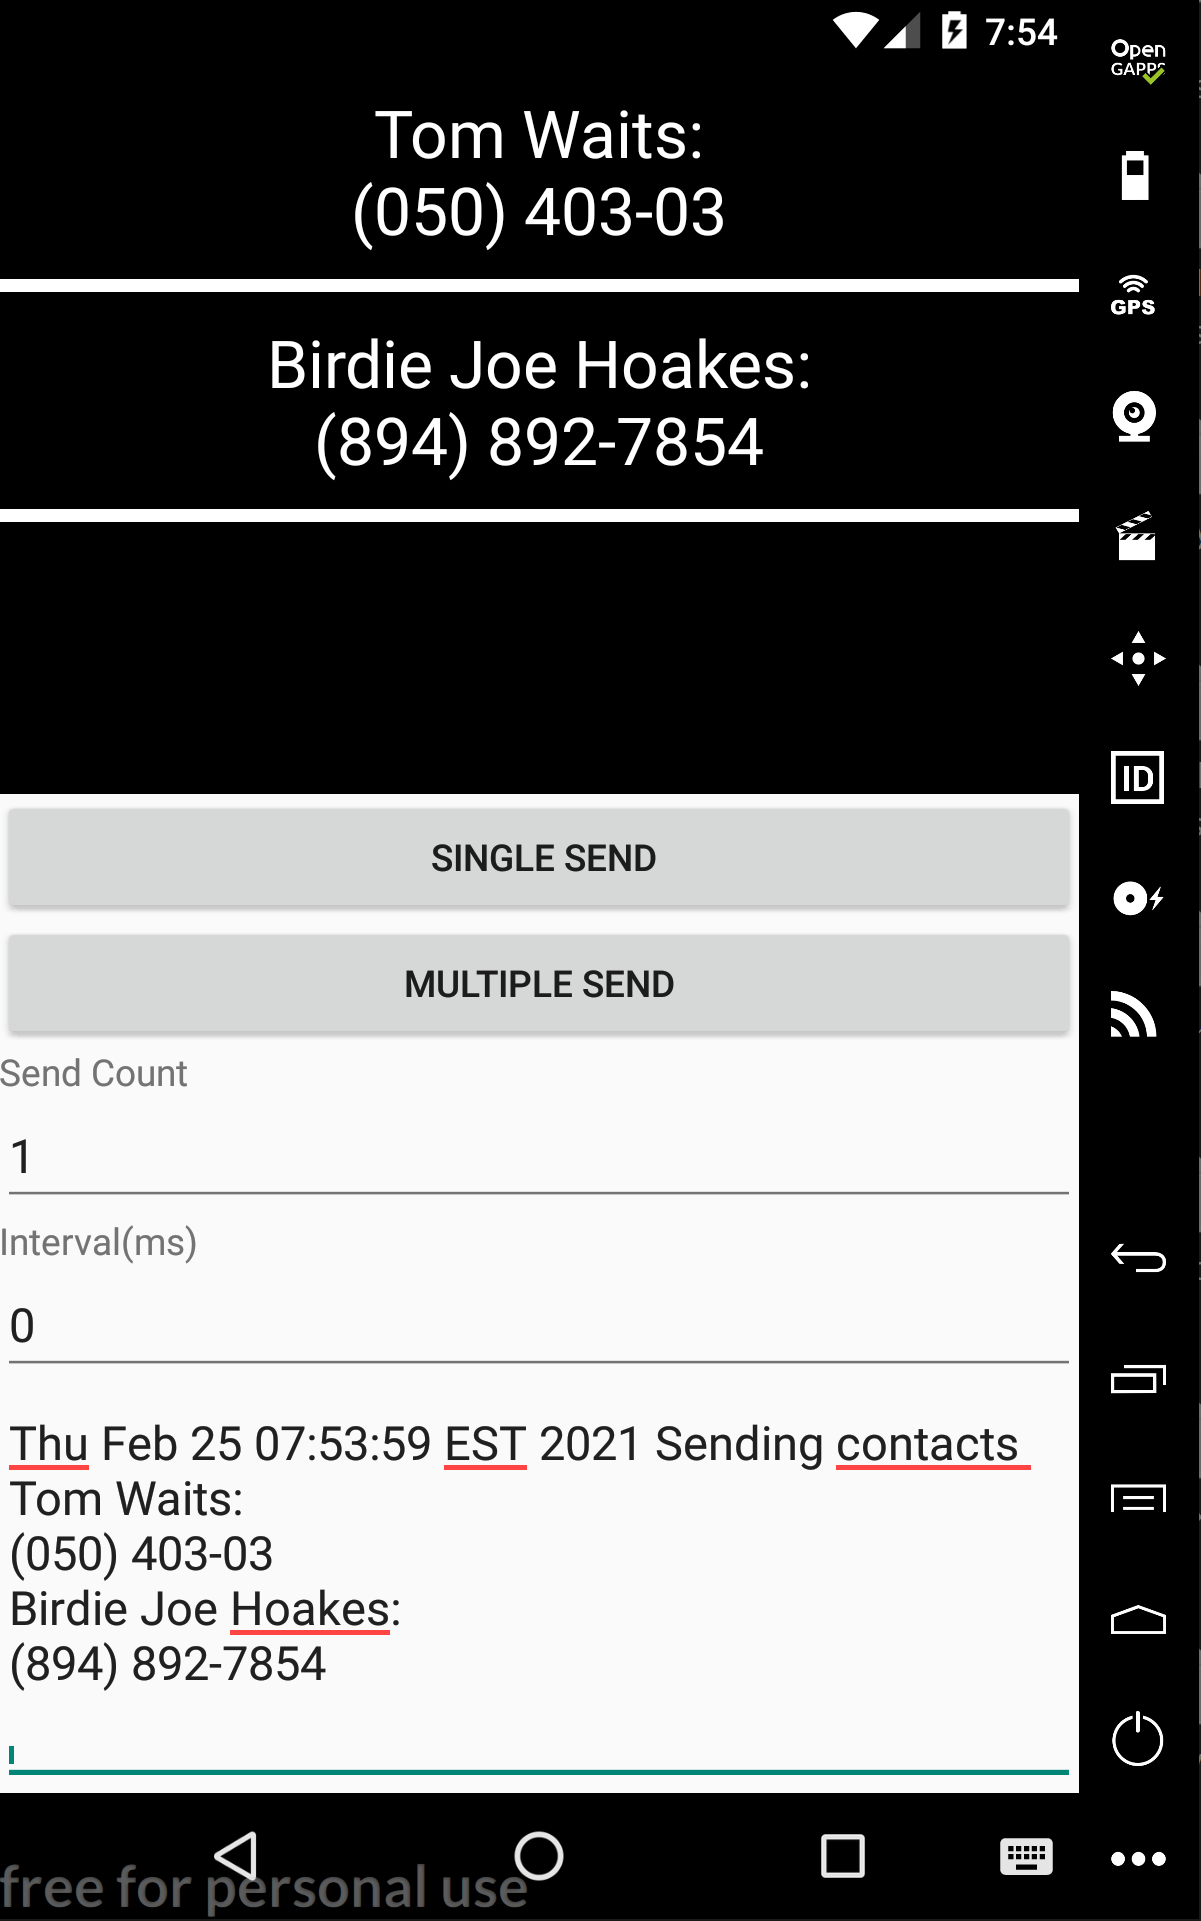
\includegraphics[height=0.5\textheight]{graphics/Reader}
	\caption{Reader}
	\label{fig:readerGUI}
	\end{subfigure}
\hfill	
	\begin{subfigure}[h]{0.5\textwidth}
	\centering
	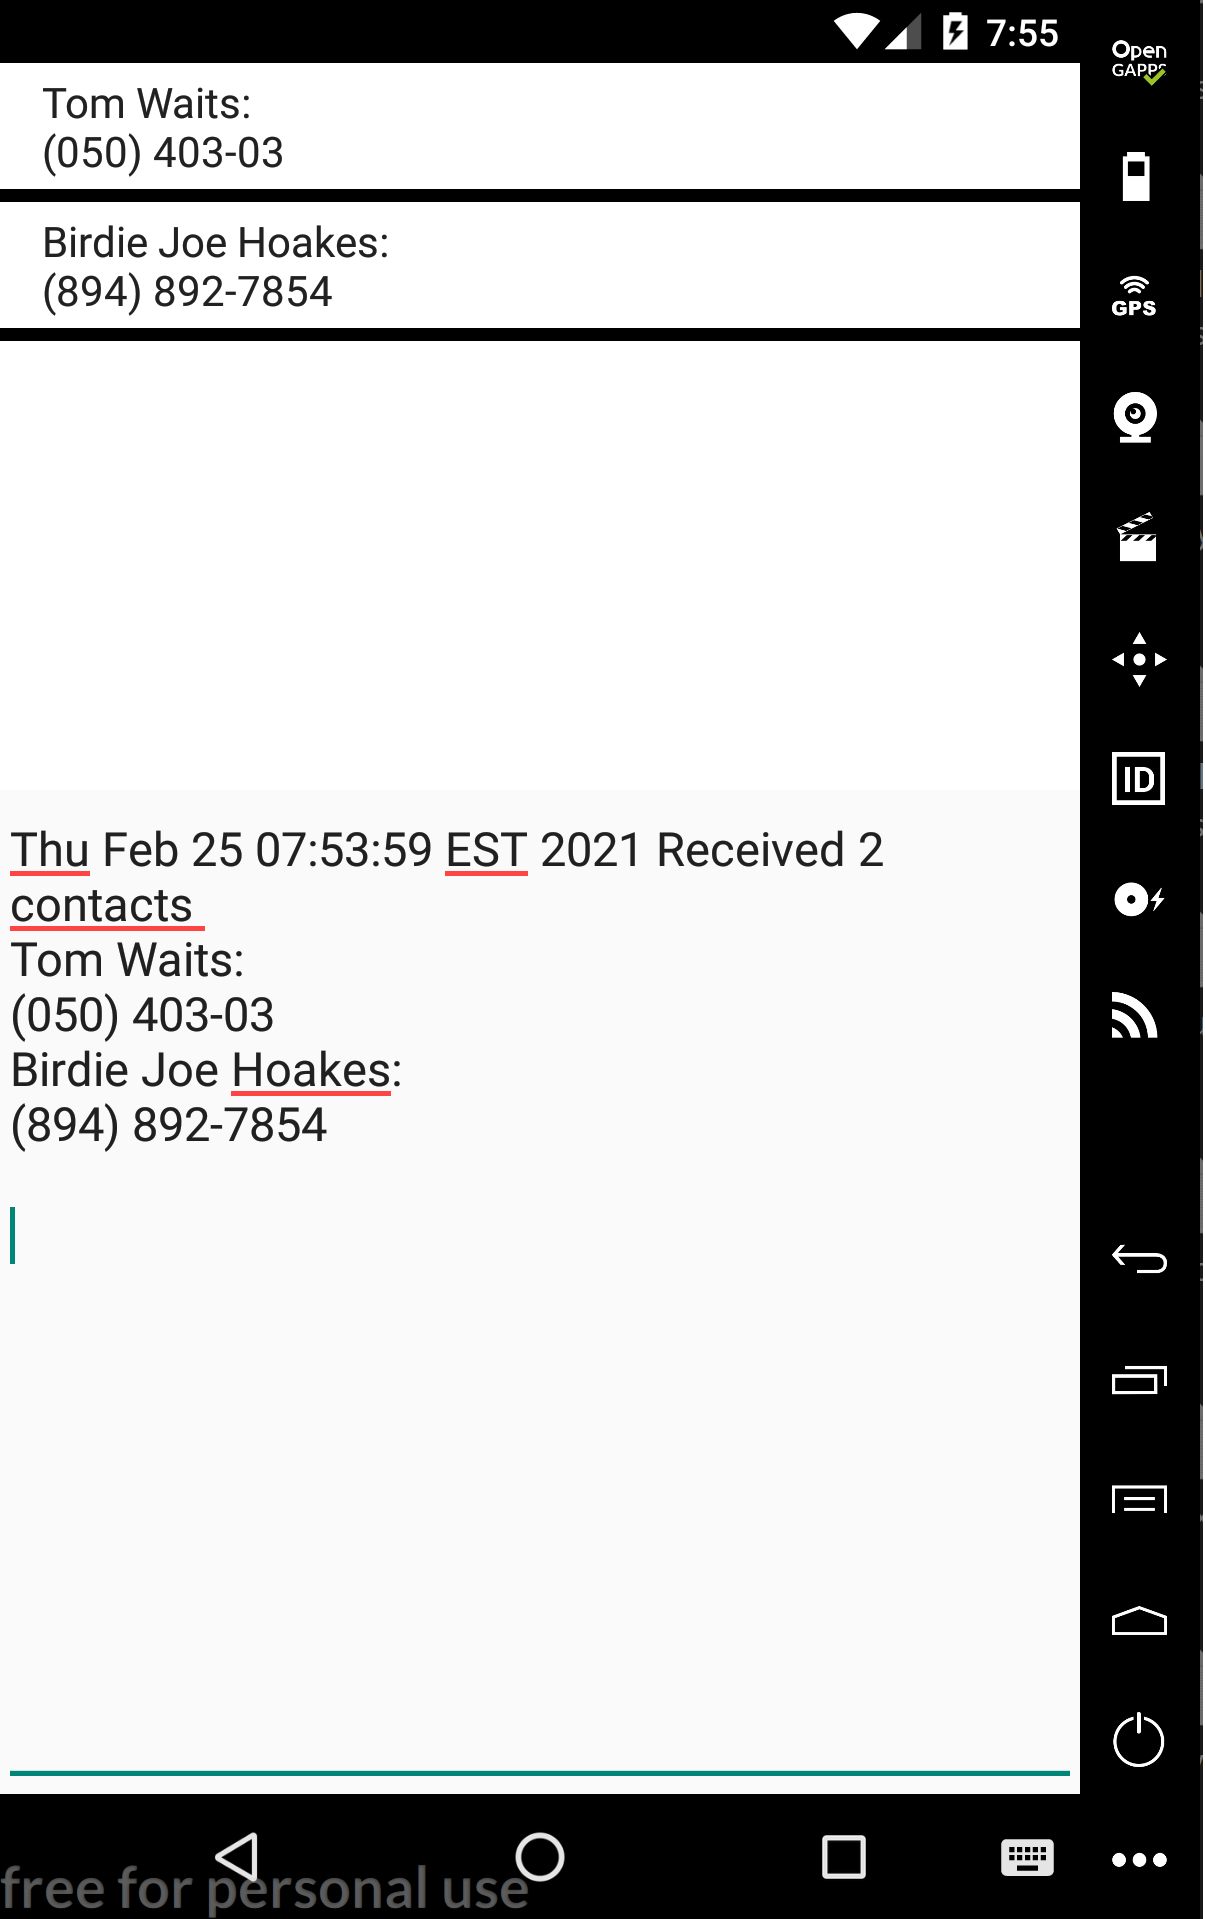
\includegraphics[height=0.5\textheight]{graphics/Publisher}
	\caption{Publisher}
	\label{fig:publisherGUI}
	\end{subfigure}
\caption{Reader \& Publisher GUI}
\label{fig:readerPublisherGUI}
\end{figure}

The reader application reads the contacts list on the Android device and sends it to the publisher via an intent.  The publisher displays what it receives on the screen. The two applications do this using the O/S methods we are interested in monitoring from section \ref{sec:OSMethodsOfInterest}.  The interceptor module that is embedded into the reader and publisher at runtime, recognises when they call the methods of interest and notifies the monitor via intents.  The monitor hosts the very same implementation of the \RH\ algorithm used in the functional testing, we simply placed that code into the monitor and added the ability to receive intents from the interceptor.

All components of this test environment were developed in Java using the Android Studio IDE.  Links to the source code for the reader and publisher apps, the interceptor and the standard \RH\ monitor are in appendices \ref{app:PerformanceTestCode}, \ref{app:InterceptorCode} and \ref{app:StandardRHMonitorCode} respectively.

\newpage

\subsection{Test Execution}
\label{subsec:PracticalPerformanceAnalysisExecution}

To understand the relationship between evaluation duration and trace length, we ran a series of ten tests where the trace length increased for each test.  The first test performed ten collusion attacks, and each subsequent test increased the number of attacks by ten until the last test performed a total of 100 attacks.  To stage multiple collusion attacks, we enhanced the reader app to read the contacts list multiple times, in a tight loop.

We used the Android Studio Profiler tool to measure the time required to evaluate a trace.  The profiler is a debug tool that works by launching the process under test on the test device and attaching to that process.  It can then measure the hardware usage of the process.  Figure \ref{fig:androidProfiler} is a screenshot of the profiler tool in operation on the monitor.  The top graph, shaded green, shows the CPU usage over time.  Memory usage over time is shown in the lower graph, shaded blue.  

To run a test, we launched the reader and publisher apps on the virtual Android device and used the profiler to launch the monitor on the virtual device.  We started the test by clicking the Multiple Send button on the reader, then watched the CPU usage of the monitor process.  The CPU usage would rise when the monitor received events from reader and publisher apps and then return to the idle level when the evaluation was complete.

The time required to evaluate the entire trace was measured as the difference between when CPU usage ramped up and when CPU usage returned to the idle level.

\begin{figure}[h!]
\centering
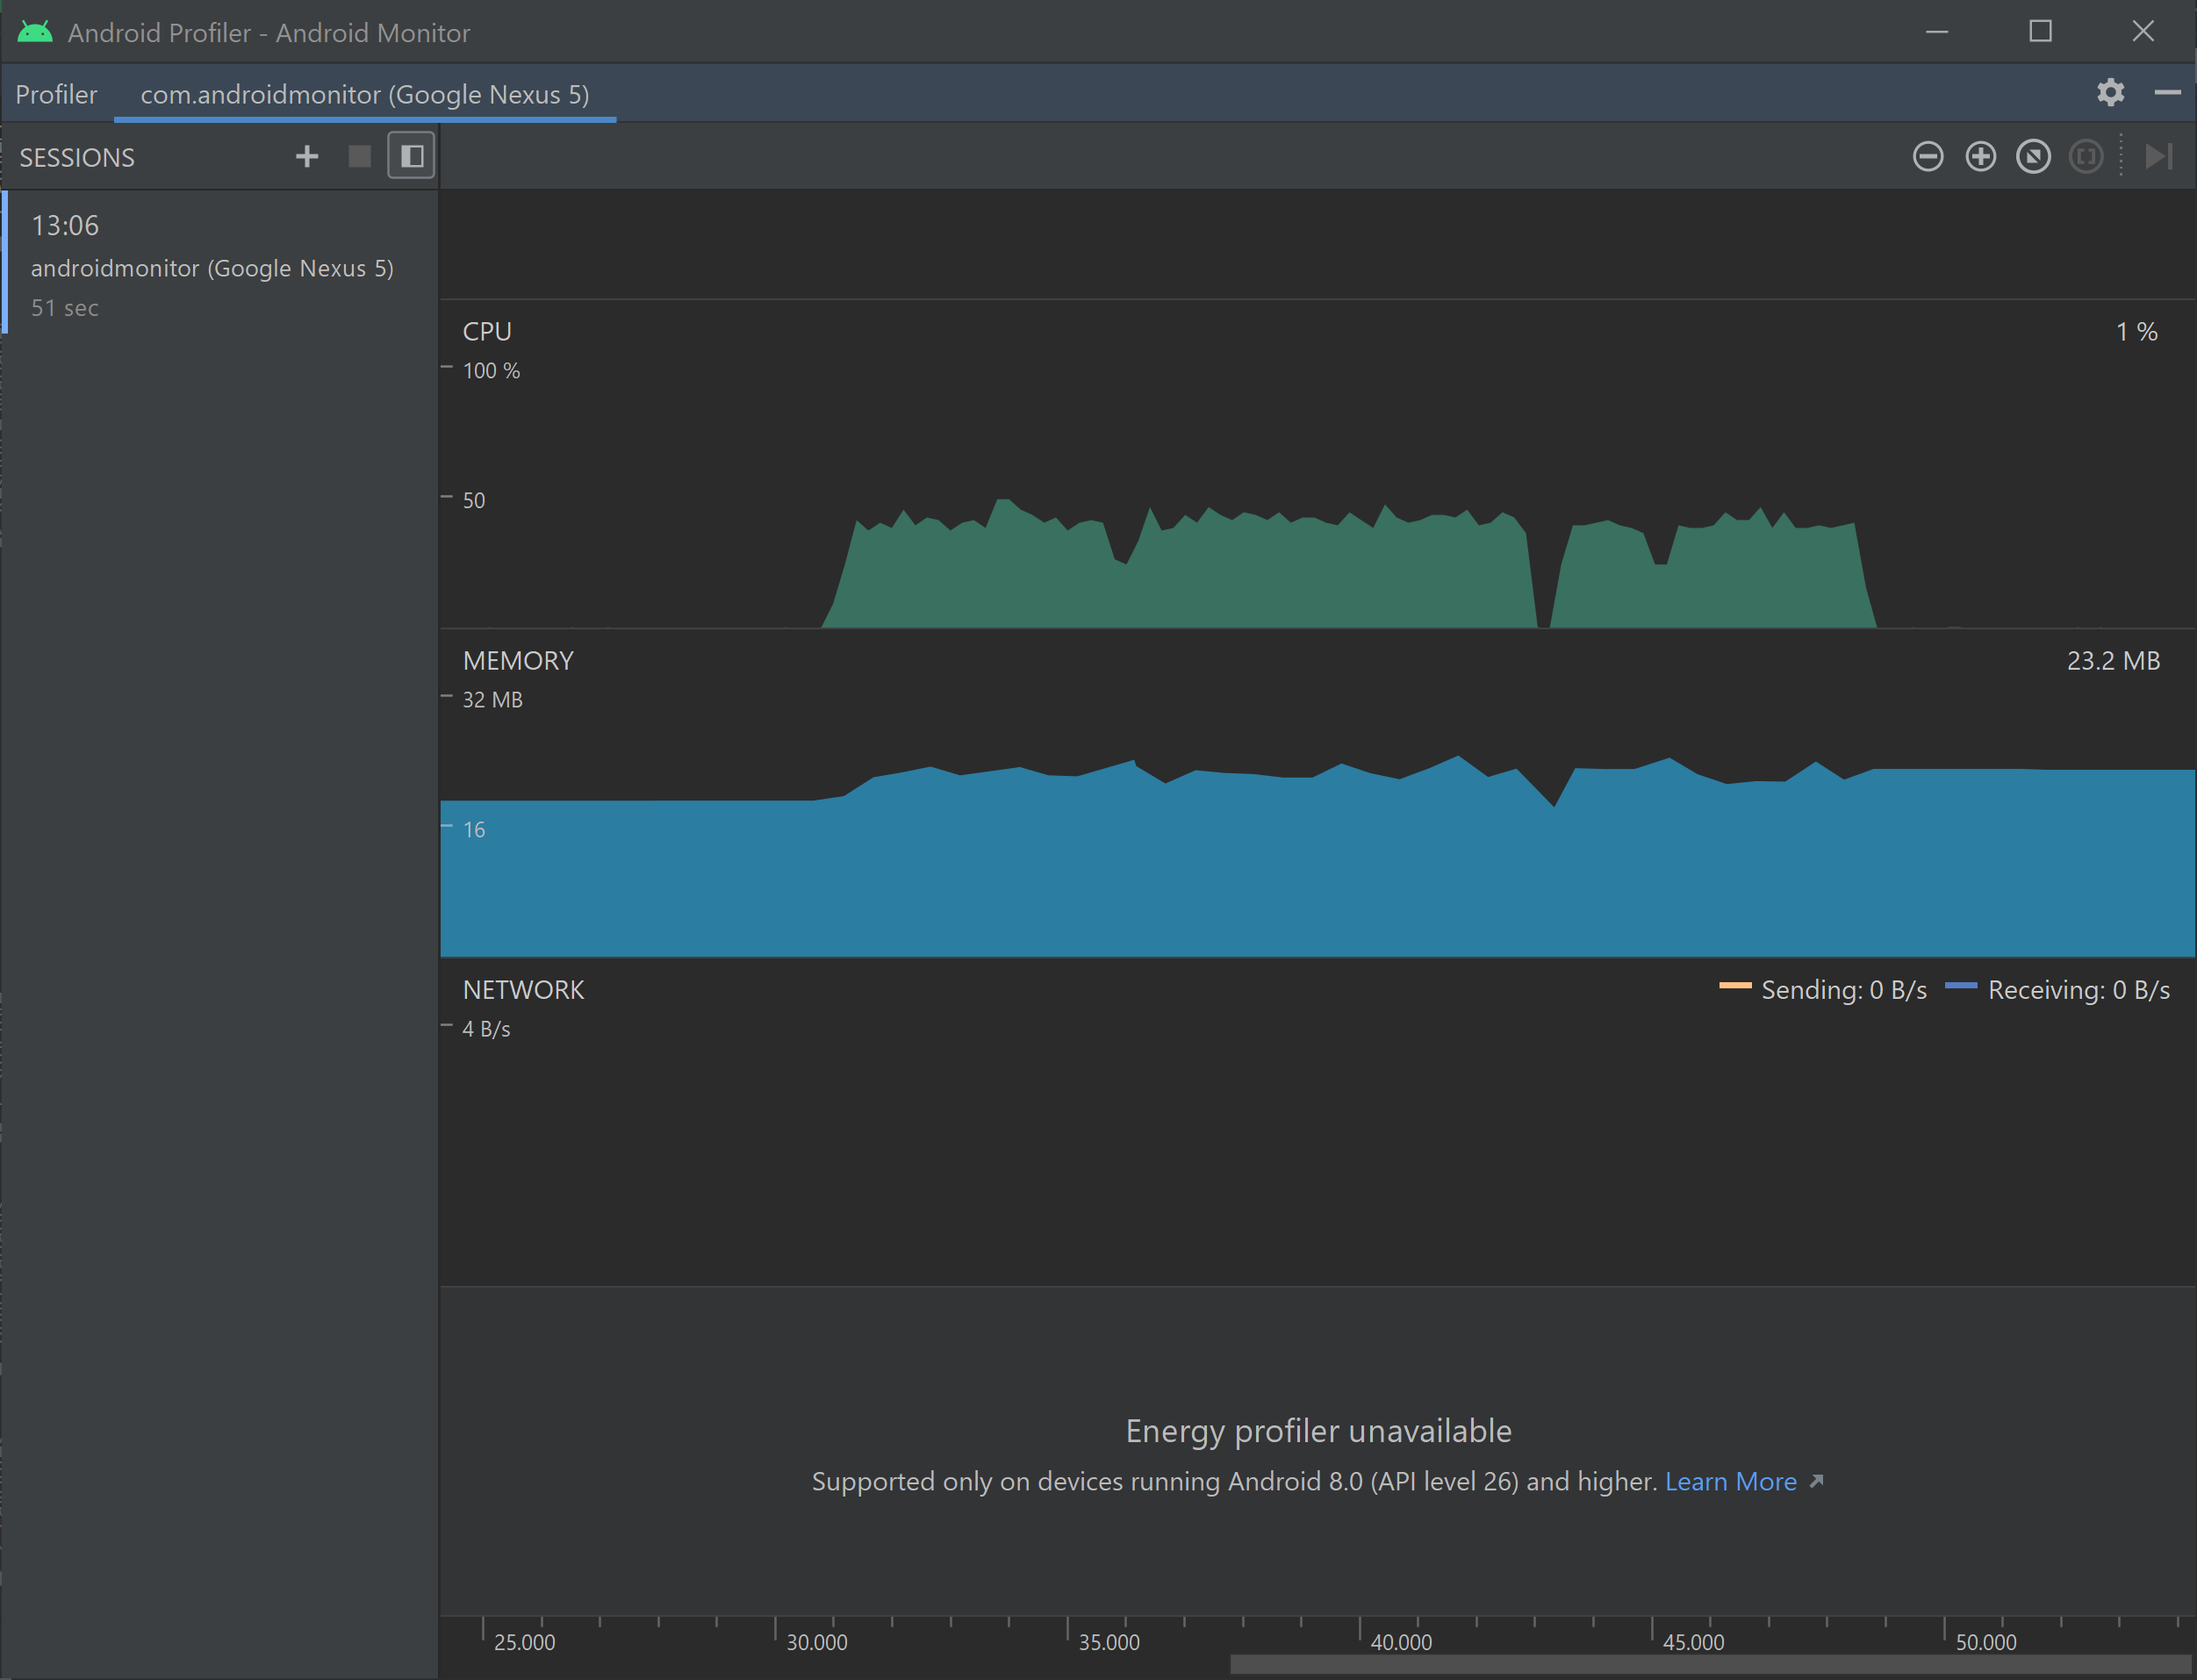
\includegraphics[width=\textwidth]{graphics/AndroidStudioProfiler3}
\caption{Profiler Tool}
\label{fig:androidProfiler}
\end{figure}

\newpage

\subsection{Test Results}
\label{subsec:PracticalPerformanceAnalysisResults}

Table \ref{tab:StandardRHExecutionTimes} shows the number of seconds elapsed when evaluating traces of increasing length.  Each row in the table is the result of a test where the trace length is greater than that of the previous test.

\begin{table}[h!]
	\centering
	\captionsetup{width=0.6\linewidth, justification=centering}
	\begin{tabular}{r|r} 
	Trace Length  & Duration\\
	(collusion sequences) & (seconds)\\
	\hline
	10 & 17\\
	20 & 72\\
	30 & 145\\
	40 & 203\\
	50 & 326\\
	60 & 462\\
	70 & 692\\
	80 & 941\\
	90 & 1198\\
	100 & 1449\\
	\hline
	\end{tabular}
	\caption{Duration of the \RH\ Algorithm Evaluating Traces of Increasing Length}
	\label{tab:StandardRHExecutionTimes}
\end{table}

\section{Scalability and Performance of the \RH\ Algorithm}
\label{sec:ScalabilityOfRosuHavelund}

Graph \ref{tab:StandardRHEvaluationDuration}, below, presents the actual test results alongside the theorised duration.  The blue curve plots the measured duration, and the red curve plots the theorised number of computational steps.  We can see that while the two curves are not precisely the same, there is a correlation between the measured duration and the theorised number of computational steps.  The measured duration curve confirms our conjecture from section \ref{sec:ComplexityAnalysis} that the time required to evaluate a trace rises quadratically with trace length.

\begin{figure}[h!]
	\centering
	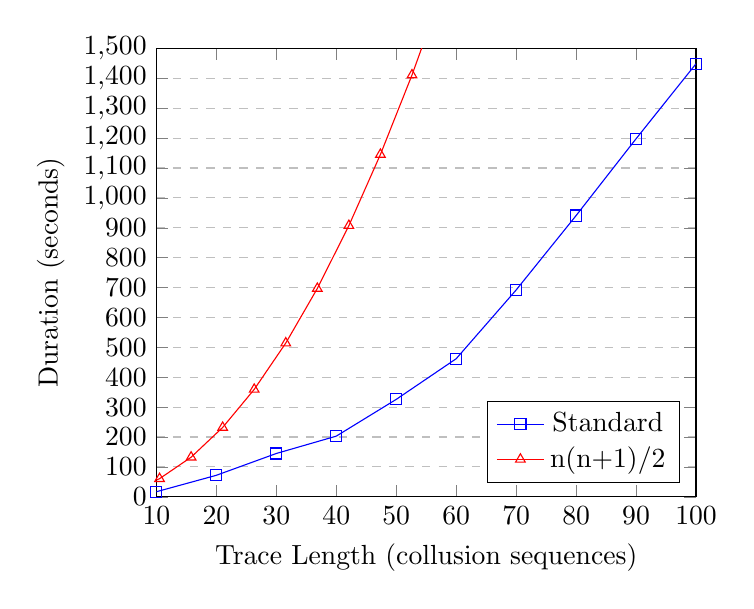
\begin{tikzpicture}
	\begin{axis}[
	    xlabel={Trace Length (collusion sequences)},
	    ylabel={Duration (seconds)},
	    xmin=10, xmax=100,
	    ymin=0, ymax=1500,
	    xtick={10,20,30,40,50,60,70,80,90,100},
	    ytick={0,100,200,300,400,500,600,700,800,900,1000,1100,1200,1300,1400,1500},
	    legend pos=south east,
	    ymajorgrids=true,
	    grid style=dashed,
	]
	
	\addplot[
	    color=blue,
	    mark=square,
	    ]
	    coordinates {
	    (10,17)(20,72)(30,145)(40,203)(50,326)(60,462)(70,692)(80,941)(90,1198)(100,1449)
	    };
	    \addlegendentry{Standard \RH}
	    
	\addplot[
	    domain=0:100, 
	    samples=20, 
	    color=red,
	    mark=triangle,
	    ]
	    {(x * (x+1)) / 2};
	    \addlegendentry{n(n+1)/2}    
	\end{axis}
	\end{tikzpicture}
	\caption{Dependency Between Trace Length and Evaluation Duration}
	\label{tab:StandardRHEvaluationDuration}
\end{figure}

When applied to realtime monitoring, the monitor should react to events as they occur and compute the outcome before the next event arises.  Otherwise, the monitor will become overwhelmed and never finish evaluating:\\

\indent Let $e_1$ and $e_2$ be two consecutive events.\\
\indent Lets denote the time interval between $e_1$ and $e_2$ with $I$.\\
\indent Lets call the computation time of the monitor $T$.\\
\indent Then we require from the monitor that $T \textless I$.\\
\\
With the \RH\ algorithm $T$ grows with the length of the trace. The trace will be recorded for an indefinite period, therefore the runtime of the \RH\ algorithm is unbounded and will eventually exceed any $I$.  For a technical system, it is realistic to have some expectation of the duration of $I$. That expectation is that there is no upper bound and the lower bound is in the order of milliseconds in the context of an operating system like Android. We estimate the minimum $I$ to be the interval between context switches plus the time to perform a context switch.

A solution to this problem might be to limit the length of the trace by removing the earliest event when a new event occurs.  But as $I$ is small, \RH\ will be limited to small traces.  And as we mentioned earlier in section \ref{subsec:ResettingTheMonitor}: If the length of the trace is limited, and the length of the attack sequence exceeds it, then the first act of the attack will have happened so far in the past that the event is no longer in the trace.  Therefore it becomes impossible to detect the attack.\\
\\
It is evident from these observations that the algorithm is not suitable for realtime monitoring.\\

%Deleting information comes at the price that monitoring is prone to miss attacks: An attack sequence comprises events corresponding to the actions of the attack.  The length of an attack sequence is unbounded, and to compound the problem, the trace may have unrelated events between the events of the attack sequence.\\
%
%\indent Let $e_n$ be the first event in an attack sequence, $e_m$ be the last event in the sequence and $n \leq m$.\\
%\indent Lets denote an attack sequence $e_n...e_m$ with $s$.\\
%\indent Lets call the trace $t$.\\
%\indent Then the monitor requires that $| s | \leq | t |$.\\
%\\